The event generators used in this work are based on the MAID unitary isobar model \parencite{Tiator2006MAIDTechniques}, \parencite{Dreschsel1992ThresholdNucleons} which concerns the photo and electroproduction of pions off of nucleons. It originated as an ``\textbf{A}mplitudes \textbf{A}nd \textbf{O}bservables '' (AAO) generator that worked in the resonance regime \parencite{Burkert1991AmplitudesGenerator} and was extended to function at higher W based on theoretical models \parencite{Goloskokov2010AnElectroproduction} and validated on experimental data \parencite{Bedlinskiy2014ExclusiveCLAS} as well as used in recent physics results \parencite{Diehl2022MultidimensionalRegion}. 

There are two generators, ``aao\_norad'', which is a nonradiative generator that creates events with an outgoing electron, proton, and two photons from the decay of the neutral pion, and ``aao\_rad'', which incorporates radiative corrections into the event generation and produces events with an outgoing electron, proton, neutral pion, and radiated photon. These two generators were refactored to function under a larger software package \href{https://github.com/JeffersonLab/aao_gen}{aao\_gen} which provides access to both generators in one system. Sample distributions of the nonradiative generator are shown in \ref{fig:aao_norad_gen}.

    \begin{figure}[H]
        \centering
        \subfloat{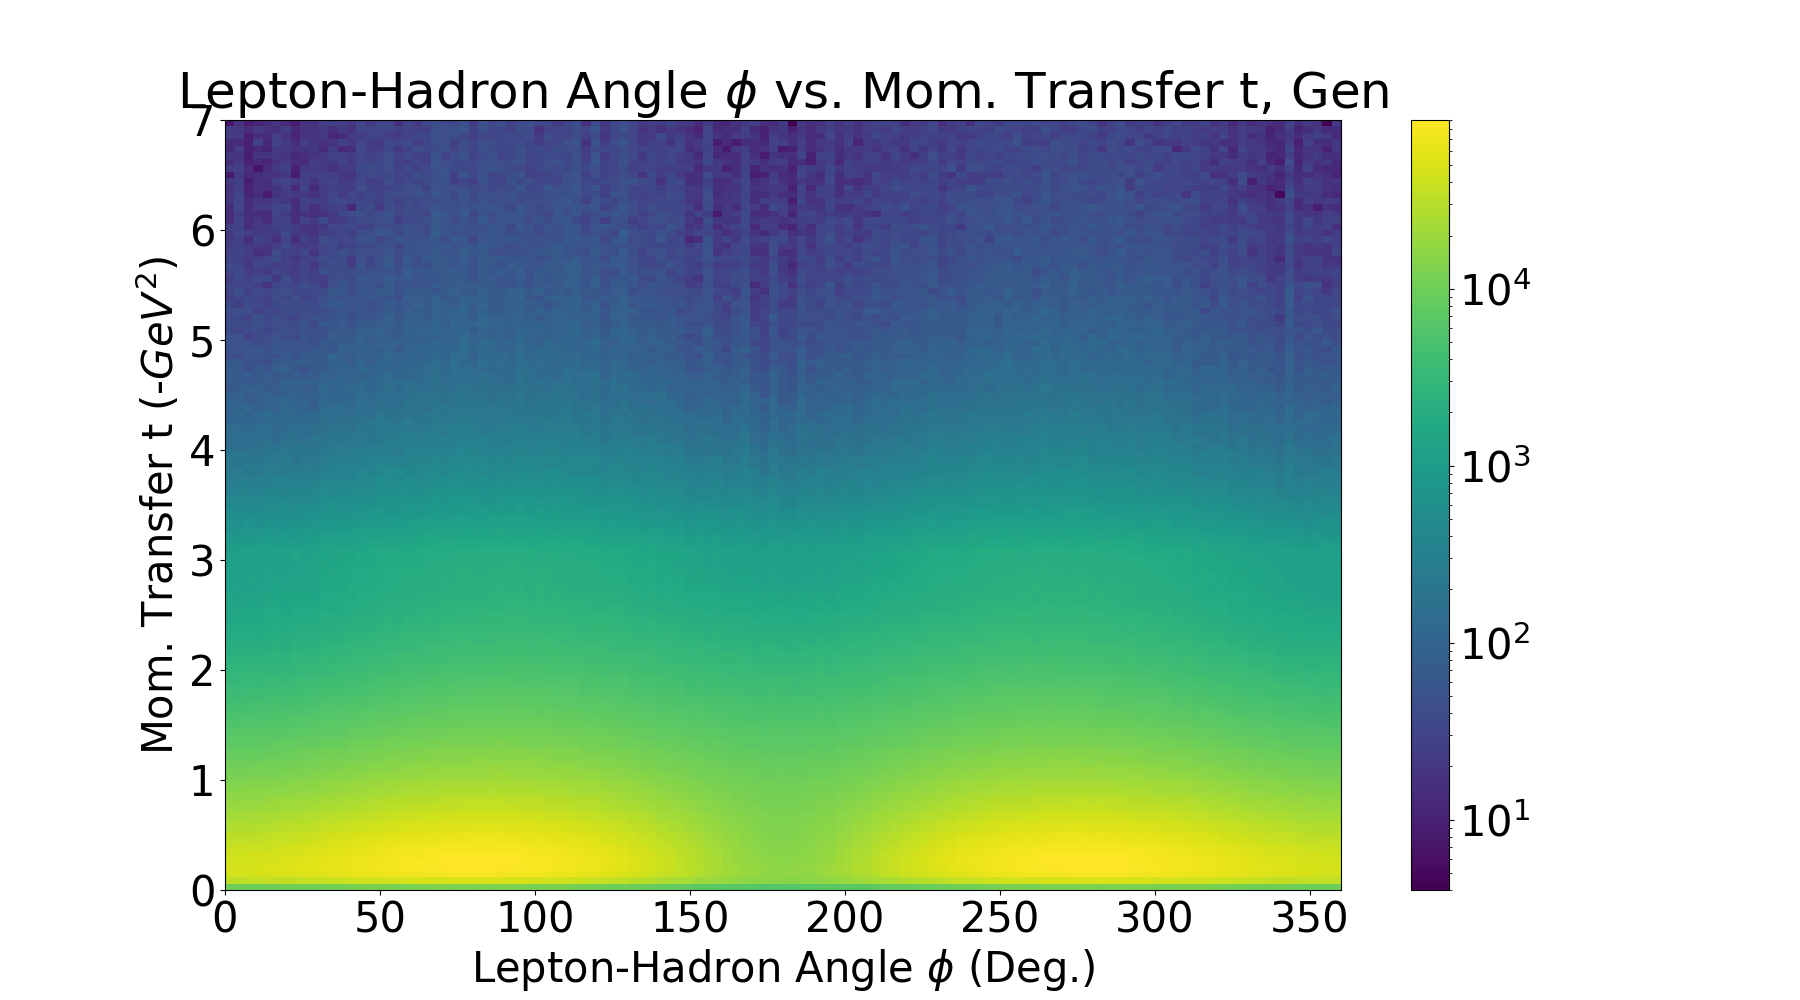
\includegraphics[width=0.5\textwidth]{Chapters/Ch3-Simulations/event_generation/pics/Lepton-Hadron_Angle_phi_vs_Mom_Transfer_t,_Gen.png}}
        \hfill
        \subfloat{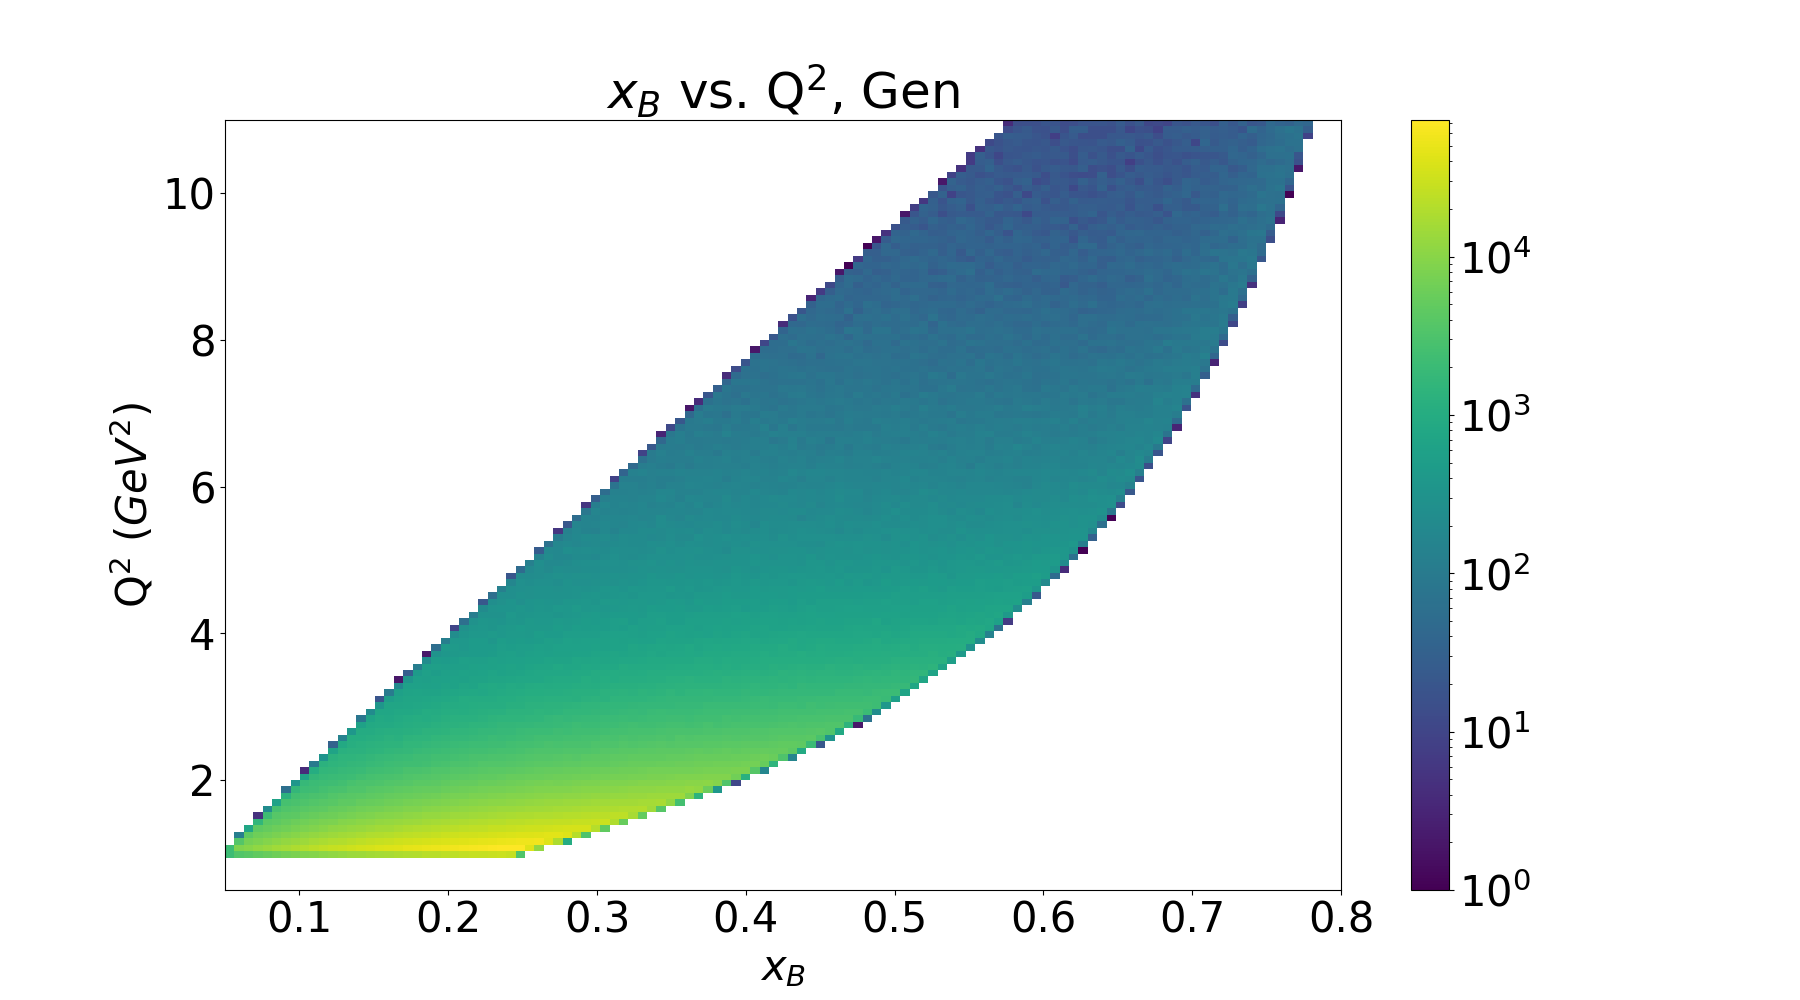
\includegraphics[width=0.5\textwidth]{Chapters/Ch3-Simulations/event_generation/pics/x_B_vs_Q2,_Gen.png}}
        \caption[Generated Event Distributions]{Generated event distributions over the 4 kinematic variables used in this work.}\label{fig:aao_norad_gen}
    \end{figure}


The radiative generator builds on the nonradiative generator to include Radiative Corrections (RC). The generator calculates s-peak and p-peak radiative corrections according to the Mo/Tsai scheme \parencite{MO1969RadiativeScattering}. The calculation produces a radiated photon with a distribution as shown in \figref{fig:aao_rad_mom_distribution}. While more realistic than the nonradiative generator, it also takes roughly 100 times as long to produce events, and so in practice both generators are utilized. 


    \begin{figure}
        \centering
        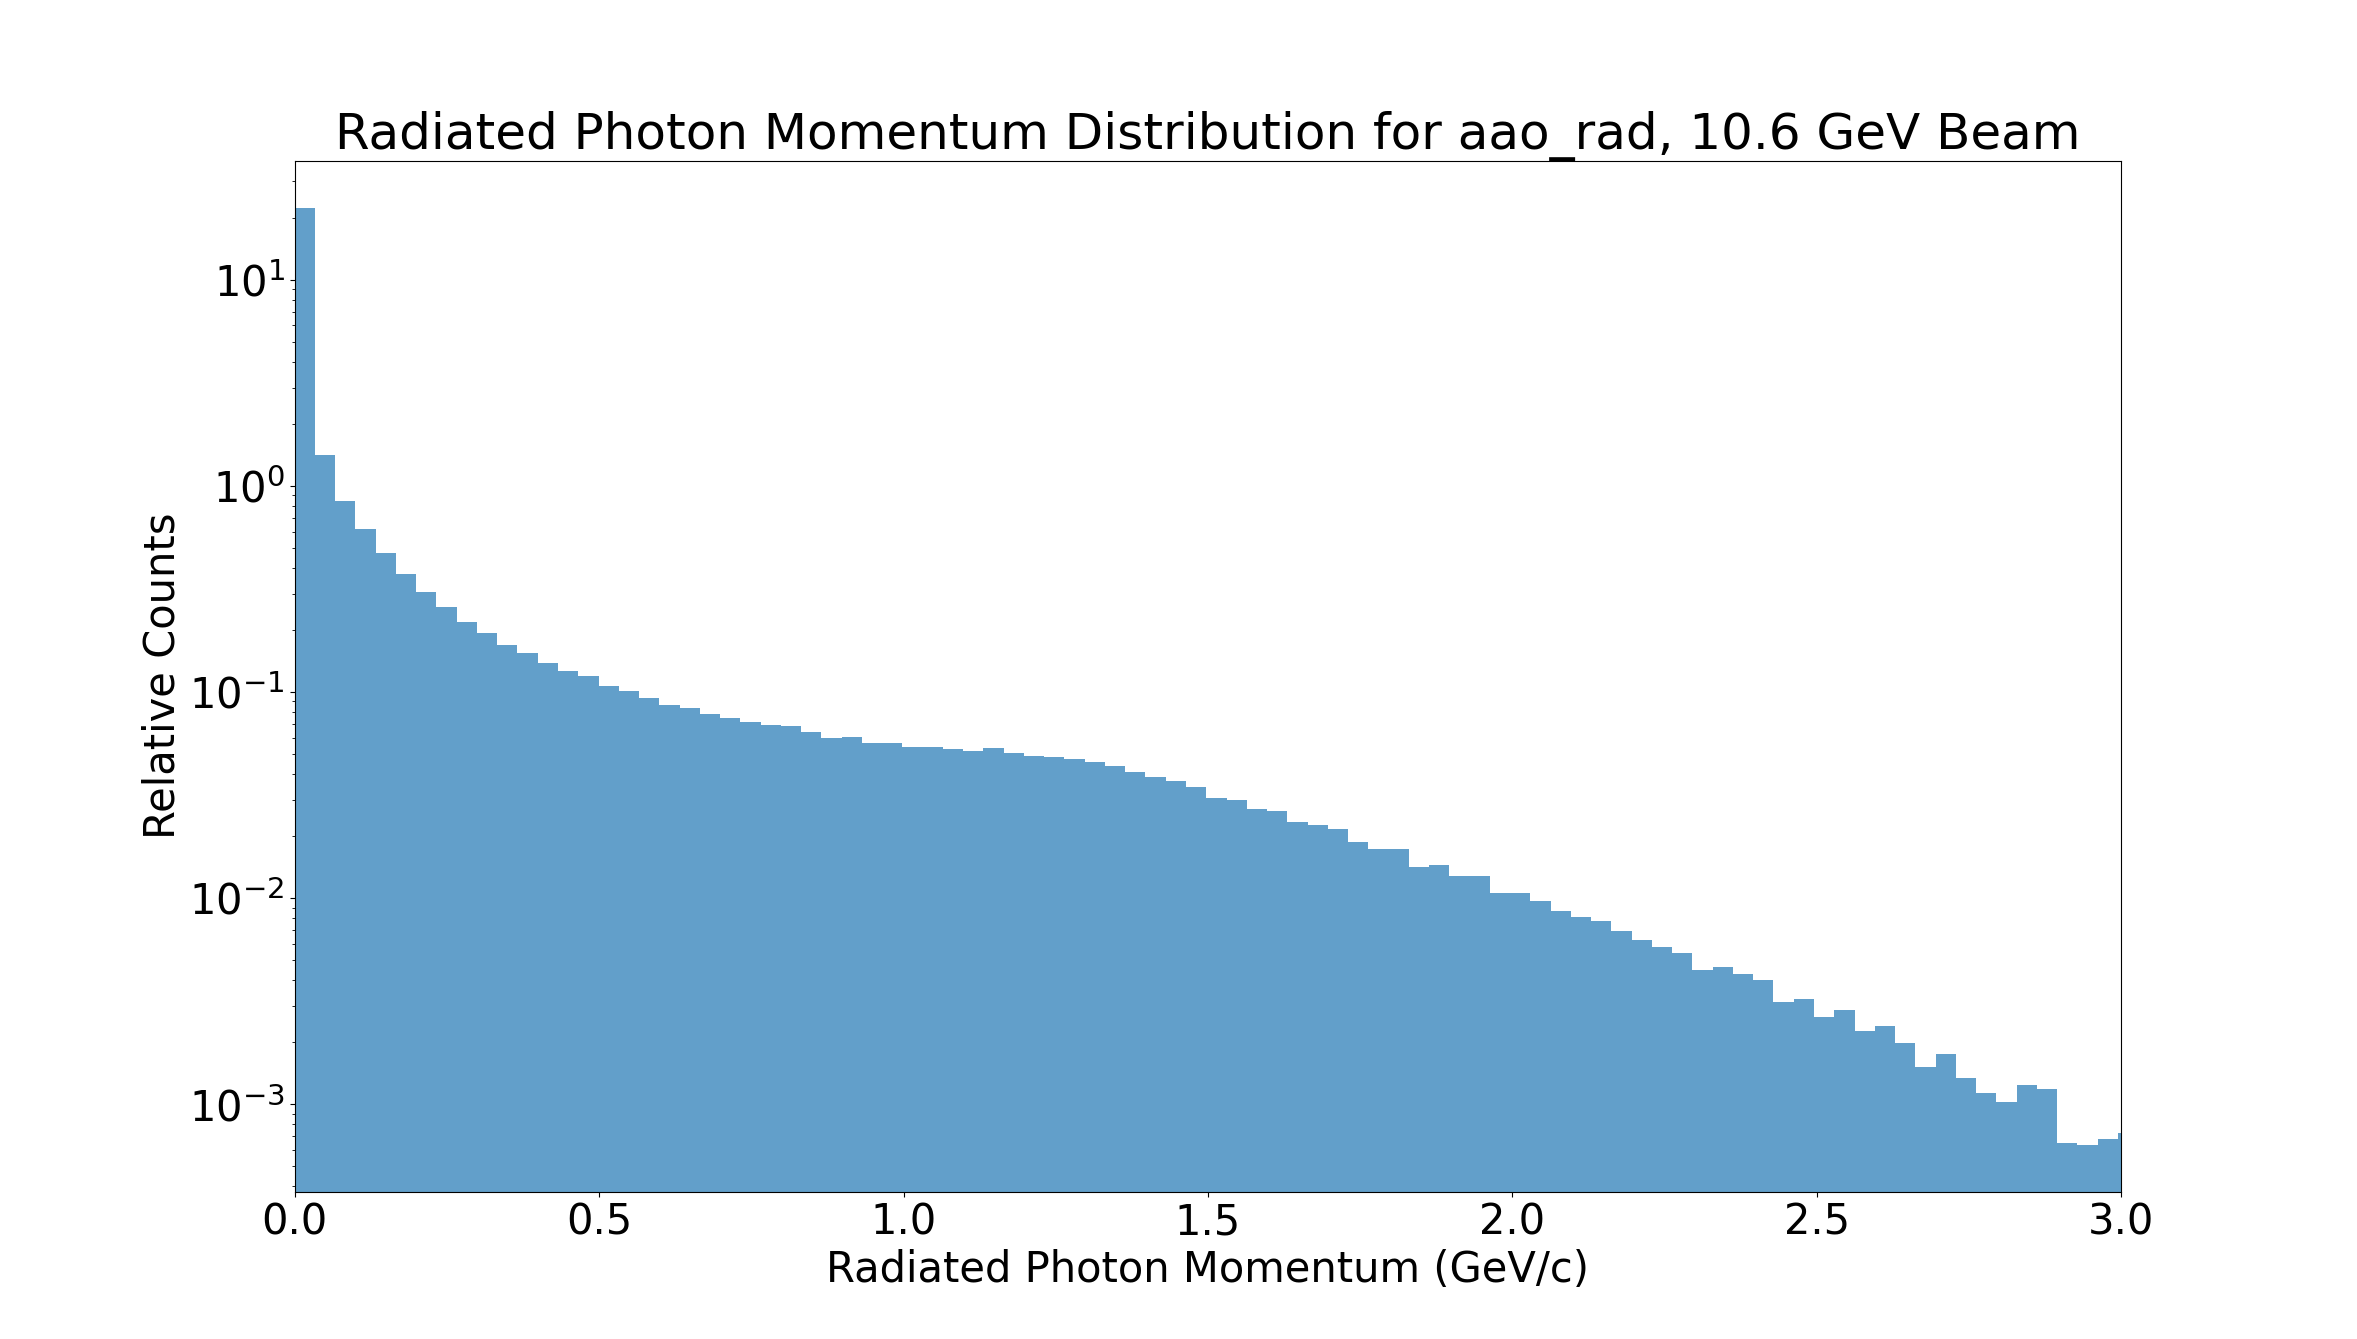
\includegraphics[trim={2cm 1.25cm 2cm 2.5cm},clip,width=0.879\textwidth]{Chapters/Ch3-Simulations/event_generation/pics/radiated_photon_momentum.png}
        \caption[aao\_rad radiated photon momentum distribution]{aao\_rad radiated photon momentum distribution. The horizontal axis is the radiated photon momentum, in units of Gev/c.}
        \label{fig:aao_rad_mom_distribution}
    \end{figure}
    
%AAO rad genreates four particles, an electron (PID 11), proton(PID 2212), radiated photon (22), and produced pion  (111)
    

%// Pi0 leptoproduction in Goloskokov-Kroll (GK) model. The code is currently being tested and implemented in PARTONS framework with additional features. If you plan to use this work in a publication, please use and reference the most recent version of PARTONS in http://partons.cea.fr 
\iffalse
% NOTES FROM VALERY KUBEROSKSKY
Andrey Kim and Nick Markov have the pi0 generator. It has my parametrization for W>2 GeV and MAID for W<1.7 GeV.

My model will for sure work for 12 GeV. It actually very close even for the COMPASS pi0 data (180 GeV muon beam).

There is reasonable coincidence between my model and MAID in the point W=1.7 GeV, not ideal but good enough for the MC.

I think actually that my parametrization has to work in the region W<2 GeV but I am not sure that MAID is doing good job due to the absence the experimental data at W~1.7 GeV. 

%FROM ONE OF THE READMES:
***************************************************************************
*      AUTHOR:        V. BURKERT AND Z. LI
*      FIRST VERSION: SUMMER, 1991.  RECENT UPDATE: MAY.1993
* AO IS WRITTEN BASED ON THE ORIGINAL PROGRAM A_AND_O FROM V.BURKERT
* THIS PROGRAM SHOULD BE LINKED TO EITHER QKMC OR QKXM FOR THE CALCULATION
* OF QUARK MODEL.  
* QKMC AND QKXM USE DIFFERENT FORM FACTORS:
* QKMC USES THE TREATMENT OF FOSTER ET. AL.
* QKXM USES THE DIPOLE FORM FACTOR 
* QKMC IS THE DEFAULT CHOICE IN THIS PACKAGE.
* AO CAN BE USED TO EXAM: Q2-DEPENDENCE OF HELICITY AMP. AT RES. POSITION (GO1)
*                         OUTPUT:GDH.TOP: A B CA(A_1/2) CB(A_3/2)
*                         GDH SUM RULE (GO2):OUTPUT GDH.TOP
*                         OBERVABLES  (RETURN):OUTPUT TEST.TOP
**************************************************************************
*           AO.FOR
* AO CONTAINS THE FOLLOWING SUBROUTINES/FUNCTIONS:
* SIGMA--CALCULATES OBSERVABLES
* EPRES--CALCULATES BREIT-WIGNER RESONANCE AMPLITUDES
* EXPA --CALCULATES THE HELICITY AMPLITUTES FROM EXPT (V.BURKERT ORIGINAL)
* BORNT--CALCULATES THE BORN TERM CONTRIBUTIONS
* BACK --CALCULATES BORN AND NON-BORN BACK GROUND TERMSS
* QKMA --CALCULATES THE HELICITY AMPLITUTES FROM QUARK MODEL
* RAMPF --CALCULATES THE Q2-DEPENDENCE OF THE HELICITY AMP. AT RES. POSITIONS
* HAMP --CALCULATES THE ENERGY-DEPENDECE OF THE RESONANCE HELICITY AMPLITUDES
* QKMC --CALCULATES THE COUPLING CONSTANTS FROM QUARK MODEL
************************************************************************
**************************************************************************
* UPDTATED: NOV., 1992
*         * WITH NEW OPTIONS TO TURN THE BORN TERM ON AND OFF
*         * BORN TERM ARE MODIFIED WITH A CUT OFF FACTOR AT HIGHER 
*           ENERGIES (WCM>1.3 GEV)
*         * SOME CORRECTIONS HAVE BEEN MADE TO THE EXPA SUBROUTINE
***************************************************************************  

 %OTHER GENERATOR NOTES:
    For Exclurad we have similar model, in end may have to iterate a few times to improve the model
    Exlclurad specifically for resonance region, theoretically should be correct, input probably needs to be updated, can put Valery’s new parameterization to cover higher range. Should not be a real issue to implement it because same thing was done for AAORad. High q2 cannot be covered because parameterization only goes to CLAS6 range
    FX: the cruicail thing is to fold in the radiative corrections with acceptance and efficiens. Best mothod is to use fast monte carlo


    aao\_rad and aao\_norad are event generators for exclusive pi0 and pi+ channels with/without radiative effects.  They are written in Fortran.  The program was initially developed by Volker Burkert long time ago for the resonance region, then has been evolved for many years and recently extended to DIS region even though lots of things need to be done.  Try this to see whether it works.  
\fi

\iffalse

    \subsection{Nonradiative Generator}
            Include generator plots, specitics of layout
    

    \subsection{Radiative Generator}
     % Include generator plots, specitics of layout, plots showing W cut offs, etc
    %SANGBAEK PG 76 RC
\fi
   